% line, arrowhead, node


\documentclass{standalone}

%maths
\usepackage{tikz}
\usepackage{scalerel}
\usepackage{pict2e}
\usepackage{tkz-euclide}
\usetikzlibrary{calc}
\usetikzlibrary{patterns,arrows.meta}
\usetikzlibrary{shadows}
\usetikzlibrary{external}

%pgfplot

\usepackage{pgfplots}
\pgfplotsset{compat=newest}
\usepgfplotslibrary{statistics}
\usepgfplotslibrary{fillbetween}

%colours
\usepackage{xcolor}



\begin{document}



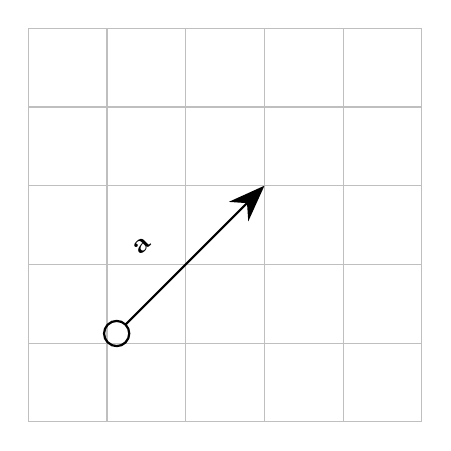
\begin{tikzpicture}

\draw[step = 1,  lightgray] (0,0) grid (5,5);

\draw[thick, {Circle[scale = 2, open]}-{Stealth[scale=2]}  ] (1,1) -- (3,3) node[rotate = 45, midway, above left = 10pt] {$\mathbf{a}$};   
%draws line. -> arrow, -stealth  --> a type of arrowhead




\end{tikzpicture}


\end{document}